\documentclass[border=8pt]{standalone}
\usepackage{pgfplots}
\pgfplotsset{compat=1.18}
\begin{document}
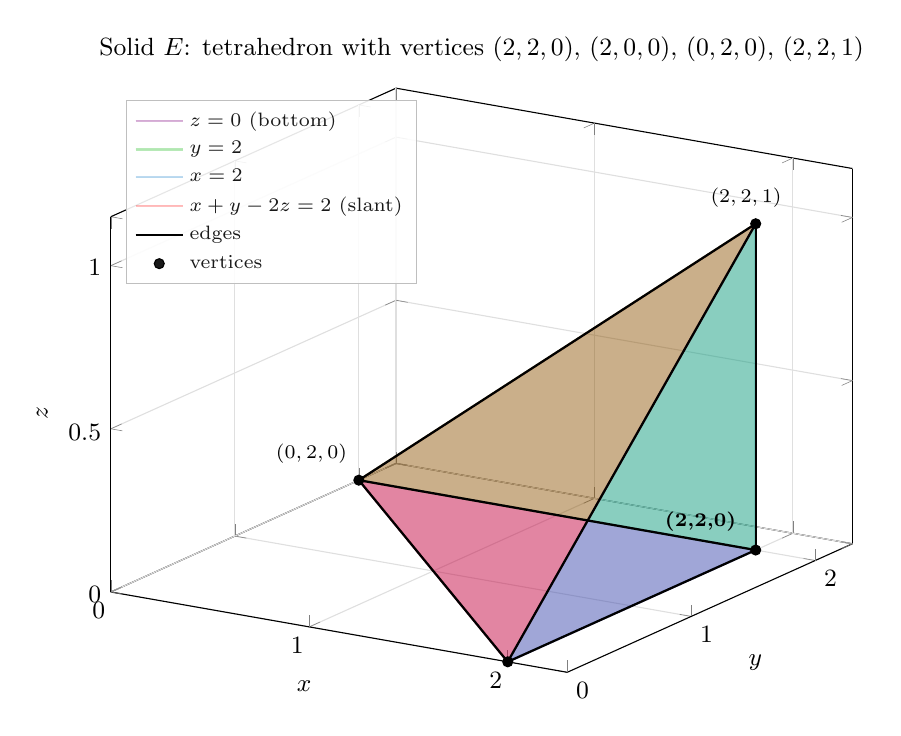
\begin{tikzpicture}[font=\small]
\begin{axis}[
    width=11cm, height=9cm,
    view={32}{22},
    xlabel=$x$, ylabel=$y$, zlabel=$z$,
    xmin=0,xmax=2.3, ymin=0,ymax=2.3, zmin=0,zmax=1.15,
    xtick={0,1,2}, ytick={0,1,2}, ztick={0,0.5,1},
    grid=major, grid style={gray!25},
    axis background/.style={white},
    title={\small Solid $E$: tetrahedron with vertices $(2,2,0)$, $(2,0,0)$, $(0,2,0)$, $(2,2,1)$},
    legend style={at={(0.02,0.98)},anchor=north west,font=\scriptsize,draw=gray!50,fill=white,fill opacity=0.9},
    legend cell align=left,
]
% ---- four bounding faces
\addplot3[fill=violet,opacity=0.30,draw=violet,thick]
  coordinates {(2,2,0)(2,0,0)(0,2,0)} -- cycle;
\addplot3[fill=green!70!black,opacity=0.28,draw=green!70!black,thick]
  coordinates {(2,2,0)(2,2,1)(0,2,0)} -- cycle;
\addplot3[fill=cyan!70!blue,opacity=0.28,draw=cyan!60!blue,thick]
  coordinates {(2,2,0)(2,2,1)(2,0,0)} -- cycle;
\addplot3[fill=red,opacity=0.25,draw=red,thick]
  coordinates {(2,2,1)(2,0,0)(0,2,0)} -- cycle;

% ---- edges in black (first one carries the legend entry)
\addplot3[black,thick,no marks] coordinates {(2,2,0)(2,2,1)};
\addplot3[black,thick,no marks,forget plot] coordinates {(2,2,0)(2,0,0)};
\addplot3[black,thick,no marks,forget plot] coordinates {(2,2,0)(0,2,0)};
\addplot3[black,thick,no marks,forget plot] coordinates {(2,2,1)(2,0,0)};
\addplot3[black,thick,no marks,forget plot] coordinates {(2,2,1)(0,2,0)};
\addplot3[black,thick,no marks,forget plot] coordinates {(2,0,0)(0,2,0)};

% ---- vertices
\addplot3[only marks,mark=*,mark size=1.8pt,black] coordinates {(2,2,0)(2,2,1)(2,0,0)(0,2,0)};

\legend{$z=0$ (bottom),$y=2$,$x=2$,$x+y-2z=2$ (slant),edges,vertices}

\node[anchor=south east,font=\scriptsize\bfseries] at (axis cs:1.97,1.97,0.03) {(2,2,0)};
\node[anchor=south east,font=\scriptsize\bfseries] at (axis cs:2.18,2.0,1.04){$(2,2,1)$};
\node[anchor=north east,font=\scriptsize\bfseries] at (axis cs:1.98,0.06,0.02) {$(2,0,0)$};
\node[anchor=south east,font=\scriptsize\bfseries] at (axis cs:0.04,1.92,0.04){$(0,2,0)$};
\end{axis}
\end{tikzpicture}
\end{document}
